\pdfminorversion=4
\documentclass[aspectratio=169]{beamer}

\mode<presentation>
{
  \usetheme{default}
  \usecolortheme{default}
  \usefonttheme{default}
  \setbeamertemplate{navigation symbols}{}
  \setbeamertemplate{caption}[numbered]
  \setbeamertemplate{footline}[frame number]  % or "page number"
  \setbeamercolor{frametitle}{fg=white}
  \setbeamercolor{footline}{fg=black}
} 

\usepackage[english]{babel}
\usepackage[utf8x]{inputenc}
\usepackage{tikz}
\usepackage{courier}
\usepackage{array}
\usepackage{bold-extra}
\usepackage{minted}
\usepackage[thicklines]{cancel}
\usepackage{fancyvrb}

\xdefinecolor{dianablue}{rgb}{0.18,0.24,0.31}
\xdefinecolor{darkblue}{rgb}{0.1,0.1,0.7}
\xdefinecolor{darkgreen}{rgb}{0,0.5,0}
\xdefinecolor{darkgrey}{rgb}{0.35,0.35,0.35}
\xdefinecolor{darkorange}{rgb}{0.8,0.5,0}
\xdefinecolor{darkred}{rgb}{0.7,0,0}
\definecolor{darkgreen}{rgb}{0,0.6,0}
\definecolor{mauve}{rgb}{0.58,0,0.82}

\title[2019-04-17-irishep-awkwardnumba]{Awkward Array: Numba}
\author{Jim Pivarski}
\institute{Princeton University -- IRIS-HEP}
\date{April 17, 2019}

\usetikzlibrary{shapes.callouts}

\begin{document}

\logo{\pgfputat{\pgfxy(0.11, 7.4)}{\pgfbox[right,base]{\tikz{\filldraw[fill=dianablue, draw=none] (0 cm, 0 cm) rectangle (50 cm, 1 cm);}\mbox{\hspace{-8 cm}
\includegraphics[height=1 cm]{princeton-logo-long.png}\hspace{0.1 cm}\raisebox{0.1 cm}{
\includegraphics[height=0.8 cm]{iris-hep-logo-long.png}}\hspace{0.1 cm}}}}}

\begin{frame}
  \titlepage
\end{frame}

\logo{\pgfputat{\pgfxy(0.11, 7.4)}{\pgfbox[right,base]{\tikz{\filldraw[fill=dianablue, draw=none] (0 cm, 0 cm) rectangle (50 cm, 1 cm);}\mbox{\hspace{-8 cm}
\includegraphics[height=1 cm]{princeton-logo.png}\hspace{0.1 cm}\raisebox{0.1 cm}{
\includegraphics[height=0.8 cm]{iris-hep-logo.png}}\hspace{0.1 cm}}}}}

% Uncomment these lines for an automatically generated outline.
%\begin{frame}{Outline}
%  \tableofcontents
%\end{frame}

% START START START START START START START START START START START START START

\begin{frame}{Knowing your audience}
\vspace{0.5 cm}
{\large I presented an ``Accelerating Python'' tutorial to non-particle physics scientists:}

\small
\begin{itemize}\setlength{\itemsep}{-0.1 cm}
\item 8 Computer Science/Software Engineering/Electrical Engineering
\item 7 Physics/Astronomy/Energy Science/Atmospheric \& Ocean Science
\item 5 Finance/Business/Political Science
\item 2 Neuroscience
\item 2 Civil Engineering
\end{itemize}

\large
\vspace{0.5 cm}
\uncover<2->{I started by showing how for-loopy code must be fundamentally rewritten to take advantage of Numpy and why it might be worth the effort.}

\vspace{0.5 cm}
\uncover<3->{\textcolor{darkblue}{Surprise!} They were {\it more comfortable} with the \mbox{vectorized form (Numpy/Pandas).\hspace{-0.5 cm}} Going the other way---from Numpy to for loops---was more of an issue.}
\end{frame}

\begin{frame}[fragile]{Knowing your audience}
\large
\vspace{0.5 cm}
Regardless of which side of the divide you start from, \textcolor{darkblue}{event-at-a-time} and \textcolor{darkblue}{operation-at-a-time} approaches are rather different and have different advantages.

\vspace{0.25 cm}
\begin{columns}[t]
\column{0.47\linewidth}
\textcolor{darkblue}{\underline{event-at-a-time}}

{\small
\begin{minted}[stripnl=false]{python}
for event in everything:
    a = step1(event)
    b = step2(a)
    write_one(b)
\end{minted}
}

\begin{itemize}
\item<2-> Good for debugging: insert breakpoints, watch variables to understand a single event.
\item<3-> Detail can obscure big picture.
\end{itemize}

\column{0.46\linewidth}
\textcolor{darkblue}{\underline{operation-at-a-time}}

{\small
\begin{minted}[stripnl=false]{python}
a = step1(everything)
b = step2(a)
write_all(b)

\end{minted}
}

\begin{itemize}
\item<4-> Composition of functions can read like natural language.
\item<5-> Indexes can be hard to align: ``error driven development!''
\end{itemize}

\end{columns}
\end{frame}

\begin{frame}{}
\vspace{1 cm}
\large
\begin{center}
Most talks on awkward-array (including this meeting) are about \\ the value of introducing \textcolor{darkblue}{operation-at-a-time} into particle physics.

\vspace{1 cm}
This talk will be about getting \textcolor{darkblue}{event-at-a-time} in Python without a speed penalty.

\vspace{0.15 cm}
\uncover<2->{\textcolor{darkorange}{\bf Programming strategy should be a {\it separate question} from performance.}}
\end{center}
\end{frame}

\begin{frame}{}
\begin{columns}
\column{1.2\linewidth}
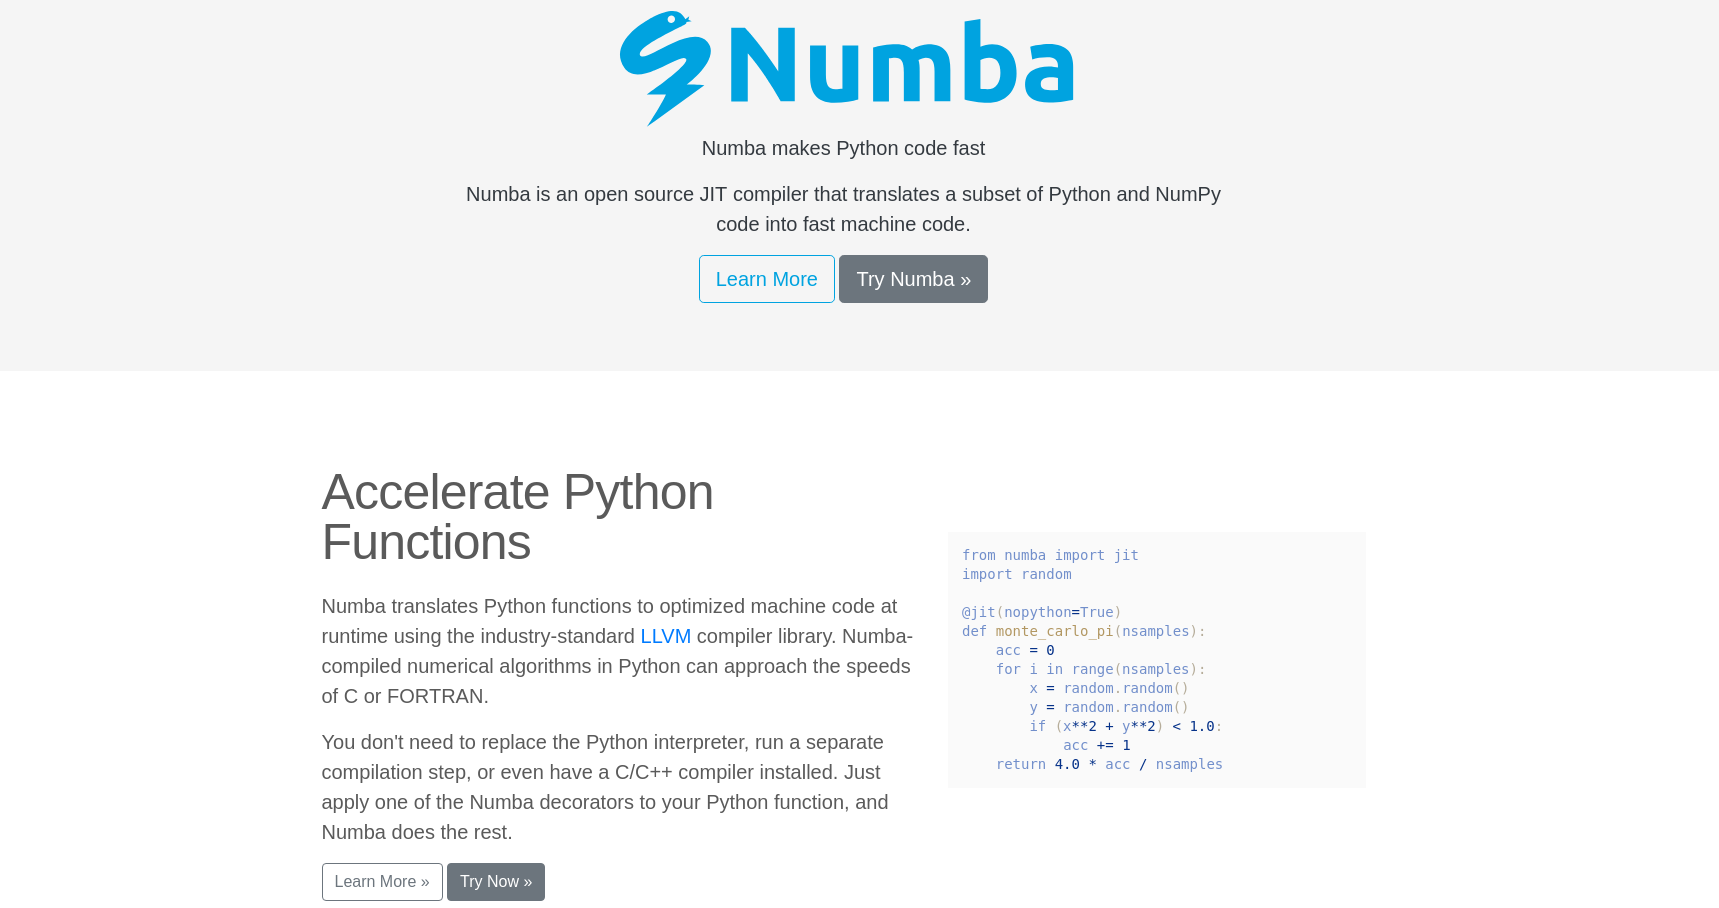
\includegraphics[width=\linewidth]{numba-website.png}
\end{columns}
\end{frame}

%% \begin{frame}{How does it differ from\ldots}
%% \large
%% \vspace{0.5 cm}
%% \begin{description}
%% \item[] PyPy, Julia, Cling; maybe this is not the place for that.
%% \end{description}
%% \end{frame}

\begin{frame}{I've been using Numba for more than 2 years\ldots}
\vspace{0.5 cm}
{\large \ldots and it always wins in my ease-of-use judgements and performance tests.}

\begin{center}
\begin{tabular}{l c r c}
{\bf Method}               & {\bf Configuration} & {\bf Speedup} & {\bf Cores} \\\hline
Plain Python               & for-loopy           &     $1\times$ & 1 \\
\textcolor{darkblue}{Numba}                      & \textcolor{darkblue}{for-loopy}           &    \textcolor{darkblue}{$50\times$} & \textcolor{darkblue}{1} \\
\textcolor{darkblue}{Numba-parallel}             & \textcolor{darkblue}{for-loopy}           &   \textcolor{darkblue}{$165\times$} & \textcolor{darkblue}{all (12)} \\
Numpy                      & columnar            &    $15\times$ & 1 \\
CuPy                       & columnar            &    $77\times$ & GPU \\
Dask                       & columnar            &    $26\times$ & all (12) \\
\textcolor{darkblue}{Numba-CUDA}                 & \textcolor{darkblue}{CUDA details}        &   \textcolor{darkblue}{$800\times$} & \textcolor{darkblue}{GPU} \\
pybind11 {\tt -O3}         & for-loopy C++       &    $34\times$ & 1 \\
pybind11 {\tt -ffast-math} & for-loopy C++       &    $90\times$ & 1 \\
Cython                     & dual language       &   $3.7\times$ & 1 \\
\end{tabular}
\end{center}

\textcolor{gray}{(Sorted by my ease-of-use judgement. Iterative fractal example in my tutorials.)}
\end{frame}

\begin{frame}[fragile]{Using Numba}
\begin{columns}
\column{1.08\linewidth}
\small
\begin{onlyenv}<1>
\begin{minted}{python}
import numpy


def run_plain(height, width, maxiterations=20):
    y, x = numpy.ogrid[-1:0:height*1j, -1.5:0:width*1j]
    c = x + y*1j
    fractal = numpy.full(c.shape, maxiterations, dtype=numpy.int32)
    for h in range(height):
        for w in range(width):             # for each pixel (h, w)...
            z = c[h, w]
            for i in range(maxiterations): # iterate at most 20 times
                z = z**2 + c[h, w]         # applying z → z² + c
                if abs(z) > 2:             # if it diverges (|z| > 2)
                    fractal[h, w] = i      # color with iteration number
                    break                  # we're done; go away
    return fractal

fractal = run_plain(6400, 9600)
\end{minted}
\end{onlyenv}
\begin{onlyenv}<2>
\begin{minted}{python}
import numpy, numba

@numba.jit
def run_numba(height, width, maxiterations=20):
    y, x = numpy.ogrid[-1:0:height*1j, -1.5:0:width*1j]
    c = x + y*1j
    fractal = numpy.full(c.shape, maxiterations, dtype=numpy.int32)
    for h in range(height):
        for w in range(width):             # for each pixel (h, w)...
            z = c[h, w]
            for i in range(maxiterations): # iterate at most 20 times
                z = z**2 + c[h, w]         # applying z → z² + c
                if abs(z) > 2:             # if it diverges (|z| > 2)
                    fractal[h, w] = i      # color with iteration number
                    break                  # we're done; go away
    return fractal

fractal = run_numba(6400, 9600)            # runs 50× faster than plain
\end{minted}
\end{onlyenv}
\end{columns}
\end{frame}

\begin{frame}[fragile]{Using Numpy}
\begin{columns}
\column{1.08\linewidth}
\small
\begin{minted}{python}
import numpy


def run_numpy(height, width, maxiterations=20):
    y, x = numpy.ogrid[-1:0:height*1j, -1.5:0:width*1j]
    c = x + y*1j
    fractal = numpy.full(c.shape, maxiterations, dtype=numpy.int32)
    z = c
    for i in range(maxiterations):         # can't break early
        z = z**2 + c                       # applying z → z² + c
        diverged = numpy.absolute(z) > 2   # |z| > 2 is "divergence"
        diverging_now = diverged & (fractal == maxiterations)
        fractal[diverging_now] = i         # only set the new ones
        z[diverged] = 2                    # clamp diverged at 2
    return fractal


fractal = run_numpy(6400, 9600)            # runs 15× faster than plain
\end{minted}
\end{columns}
\end{frame}

\begin{frame}{Here's the catch:}
\Large
\vspace{0.5 cm}
Numba can only accelerate \textcolor{darkblue}{functions} and \textcolor{darkblue}{data structures} that it recognizes (mostly numbers and arrays).

\vspace{1 cm}
\uncover<2->{They must be \textcolor{darkblue}{statically typed} (all types known before execution).}

\vspace{1 cm}
\uncover<3->{\mintinline{python}{@numba.jit(nopython=True)} only allows accelerated code; \mintinline{python}{@numba.jit()} only accelerates what it can.}
\end{frame}

\begin{frame}{We can add functions and data structures}
\vspace{0.5 cm}
\begin{columns}
\column{1.13\linewidth}
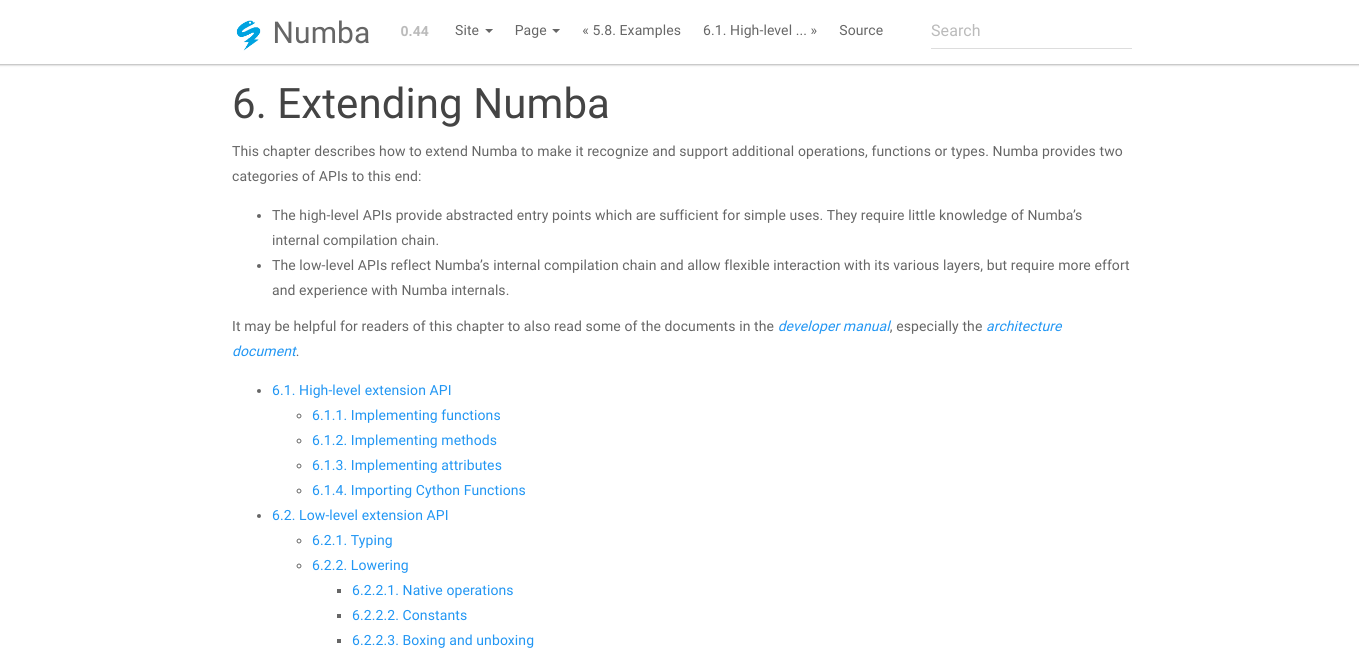
\includegraphics[width=\linewidth]{numba-extending.png}
\end{columns}
\end{frame}

\begin{frame}[fragile]{Awkward arrays are statically typed}
\vspace{0.5 cm}
Arbitrarily complex data:
{\small
\begin{minted}{python}
>>> import awkward
>>> array = awkward.fromiter(
...     [[1.1, 2.2, None, 3.3, None],
...      [4.4, [5.5]],
...      [{"x": 6, "y": {"z": 7}}, None, {"x": 8, "y": {"z": 9}}]
...     ])
\end{minted}
}

\vspace{0.5 cm}
Has a data type known before execution, which is to say, before (JIT) compilation.
{\small
\begin{minted}{python}
>>> print(array.type)
\end{minted}
\begin{verbatim}
[0, 3) -> [0, inf) -> ?((float64             |
                         [0, inf) -> float64 |
                         'x' -> int64
                         'y' -> 'z' -> int64 ))
\end{verbatim}
}
\end{frame}

\begin{frame}{}
\Large
\vspace{1.5 cm}
\textcolor{darkorange}{\bf Goal:} \textcolor{darkblue}{unbox} all array types and \textcolor{darkblue}{lower} all functions and methods, \\
so that they can be used in Numba functions written by users.

\vspace{1 cm}
\uncover<2->{\textcolor{darkorange}{\bf Status:} done with {\tt JaggedArray}, next is {\tt Table}.}

\vspace{1 cm}
\uncover<3->{\textcolor{darkorange}{\bf To use:} \vspace{0.5\baselineskip}\\ \large \mbox{\hspace{1.5 cm}\mintinline{bash}{pip install awkward-numba}} or \\ \mbox{\hspace{1.5 cm}\mintinline{bash}{conda install -c conda-forge awkward-numba}} \vspace{0.5\baselineskip}\\ and then \mintinline{python}{import awkward.numba} in Python.}
\end{frame}

\begin{frame}[fragile]{Physics-motivated example: pairs of muons and jets}
\vspace{0.15 cm}
\scriptsize
\begin{minted}{python}
import numpy, numba, awkward, awkward.numba

def random_particles(num_per_event, num_events):
    num = numpy.random.poisson(num_per_event, num_events)
    pt  = numpy.random.exponential(10, num.sum())
    eta = numpy.random.normal(0, 1, num.sum())
    phi = numpy.random.uniform(-numpy.pi, numpy.pi, num.sum())
    return (num, awkward.JaggedArray.fromcounts(num, pt),
                     awkward.JaggedArray.fromcounts(num, eta),
                         awkward.JaggedArray.fromcounts(num, phi))

num_muons, pt_muons, eta_muons, phi_muons = random_particles(1.5, 1000000)
num_jets,  pt_jets,  eta_jets,  phi_jets  = random_particles(3.5, 1000000)
\end{minted}

\vspace{0.35 cm}
\begin{uncoverenv}<2->
{\normalsize Each of these is a jagged array of particle attributes. Mass of all muon-jet pairs is}

\vspace{0.1 cm}
\begin{minted}{python}
def unzip(pairs): return pairs.i0, pairs.i1
pt1, pt2   = unzip(pt_muons.cross(pt_jets))       # make a big array of all pairs
eta1, eta2 = unzip(eta_muons.cross(eta_jets))     # separately for each attribute
phi1, phi2 = unzip(phi_muons.cross(phi_jets))     # because we don't have Tables yet

# compute mass for all muon-jet pairs in all events in one line
mass = numpy.sqrt(2*pt1*pt2*(numpy.cosh(eta1 - eta2) - numpy.cos(phi1 - phi2)))
\end{minted}
\end{uncoverenv}
\end{frame}

\begin{frame}[fragile]{Physics-motivated example: pairs of muons and jets}
\vspace{0.25 cm}

{For-loopy code to do the same thing (i.e.\ a conventional analysis):}

\scriptsize
\begin{onlyenv}<1>
\begin{minted}[stripnl=false]{python}

def run_plain(num_muons, pt_muons, eta_muons, phi_muons,
              num_jets,  pt_jets,  eta_jets,  phi_jets):
    offsets = numpy.empty(len(num_muons) + 1, numpy.int64)
    content = numpy.empty((num_muons * num_jets).sum())
    offsets[0] = 0
    for i in range(len(num_muons)):
        offsets[i + 1] = offsets[i]
        for muoni in range(num_muons[i]):
            pt1  = pt_muons[i][muoni]
            eta1 = eta_muons[i][muoni]
            phi1 = phi_muons[i][muoni]
            for jeti in range(num_jets[i]):
                pt2  = pt_jets[i][jeti]
                eta2 = eta_jets[i][jeti]
                phi2 = phi_jets[i][jeti]
                content[offsets[i + 1]] = numpy.sqrt(
                    2*pt1*pt2*(numpy.cosh(eta1 - eta2) - numpy.cos(phi1 - phi2)))
                offsets[i + 1] += 1
    return awkward.JaggedArray(offsets[:-1], offsets[1:], content)
\end{minted}
\end{onlyenv}
\begin{onlyenv}<2>
\begin{minted}[stripnl=false]{python}
@numba.jit(nopython=True)
def run_numba(num_muons, pt_muons, eta_muons, phi_muons,     # can pass JaggedArrays
              num_jets,  pt_jets,  eta_jets,  phi_jets):     # into Numba-JIT function
    offsets = numpy.empty(len(num_muons) + 1, numpy.int64)
    content = numpy.empty((num_muons * num_jets).sum())
    offsets[0] = 0
    for i in range(len(num_muons)):
        offsets[i + 1] = offsets[i]
        for muoni in range(num_muons[i]):
            pt1  = pt_muons[i][muoni]
            eta1 = eta_muons[i][muoni]
            phi1 = phi_muons[i][muoni]
            for jeti in range(num_jets[i]):
                pt2  = pt_jets[i][jeti]
                eta2 = eta_jets[i][jeti]
                phi2 = phi_jets[i][jeti]
                content[offsets[i + 1]] = numpy.sqrt(
                    2*pt1*pt2*(numpy.cosh(eta1 - eta2) - numpy.cos(phi1 - phi2)))
                offsets[i + 1] += 1
    return awkward.JaggedArray(offsets[:-1], offsets[1:], content)          # and out!
\end{minted}
\end{onlyenv}
\end{frame}

\begin{frame}{What this buys us}
\large
\vspace{0.5 cm}
\begin{center}
\begin{tabular}{l l l l}
{\bf Method} & {\bf Pro}  & {\bf Con}  & {\bf Runtime} \\\hline
{\tt JaggedArray.cross} & concise  & inflexible & \textcolor{white}{12}1.1\textcolor{white}{2} seconds \\
Plain Python loop       & explicit & verbose    & 120\textcolor{white}{.62} seconds \\
Numba-compiled          & explicit & verbose    & \textcolor{white}{12}0.62 seconds (to compile) \\
                        &          &            & \textcolor{white}{12}0.22 seconds (to run)
\end{tabular}
\end{center}

\vspace{0.25 cm}
Apart from a factor of 5 between {\tt\normalsize JaggedArray.cross} and Numba-compiled (which may leap-frog as implementations improve), we can now write arbitrary for-loop algorithms on {\tt\normalsize JaggedArray} without an enormous cost.
\end{frame}


\end{document}
